\documentclass[twoside]{book}

% Packages required by doxygen
\usepackage{fixltx2e}
\usepackage{calc}
\usepackage{doxygen}
\usepackage[export]{adjustbox} % also loads graphicx
\usepackage{graphicx}
\usepackage[utf8]{inputenc}
\usepackage{makeidx}
\usepackage{multicol}
\usepackage{multirow}
\PassOptionsToPackage{warn}{textcomp}
\usepackage{textcomp}
\usepackage[nointegrals]{wasysym}
\usepackage[table]{xcolor}

% Font selection
\usepackage[T1]{fontenc}
\usepackage[scaled=.90]{helvet}
\usepackage{courier}
\usepackage{amssymb}
\usepackage{sectsty}
\renewcommand{\familydefault}{\sfdefault}
\allsectionsfont{%
  \fontseries{bc}\selectfont%
  \color{darkgray}%
}
\renewcommand{\DoxyLabelFont}{%
  \fontseries{bc}\selectfont%
  \color{darkgray}%
}
\newcommand{\+}{\discretionary{\mbox{\scriptsize$\hookleftarrow$}}{}{}}

% Page & text layout
\usepackage{geometry}
\geometry{%
  a4paper,%
  top=2.5cm,%
  bottom=2.5cm,%
  left=2.5cm,%
  right=2.5cm%
}
\tolerance=750
\hfuzz=15pt
\hbadness=750
\setlength{\emergencystretch}{15pt}
\setlength{\parindent}{0cm}
\setlength{\parskip}{3ex plus 2ex minus 2ex}
\makeatletter
\renewcommand{\paragraph}{%
  \@startsection{paragraph}{4}{0ex}{-1.0ex}{1.0ex}{%
    \normalfont\normalsize\bfseries\SS@parafont%
  }%
}
\renewcommand{\subparagraph}{%
  \@startsection{subparagraph}{5}{0ex}{-1.0ex}{1.0ex}{%
    \normalfont\normalsize\bfseries\SS@subparafont%
  }%
}
\makeatother

% Headers & footers
\usepackage{fancyhdr}
\pagestyle{fancyplain}
\fancyhead[LE]{\fancyplain{}{\bfseries\thepage}}
\fancyhead[CE]{\fancyplain{}{}}
\fancyhead[RE]{\fancyplain{}{\bfseries\leftmark}}
\fancyhead[LO]{\fancyplain{}{\bfseries\rightmark}}
\fancyhead[CO]{\fancyplain{}{}}
\fancyhead[RO]{\fancyplain{}{\bfseries\thepage}}
\fancyfoot[LE]{\fancyplain{}{}}
\fancyfoot[CE]{\fancyplain{}{}}
\fancyfoot[RE]{\fancyplain{}{\bfseries\scriptsize Generated by Doxygen }}
\fancyfoot[LO]{\fancyplain{}{\bfseries\scriptsize Generated by Doxygen }}
\fancyfoot[CO]{\fancyplain{}{}}
\fancyfoot[RO]{\fancyplain{}{}}
\renewcommand{\footrulewidth}{0.4pt}
\renewcommand{\chaptermark}[1]{%
  \markboth{#1}{}%
}
\renewcommand{\sectionmark}[1]{%
  \markright{\thesection\ #1}%
}

% Indices & bibliography
\usepackage{natbib}
\usepackage[titles]{tocloft}
\setcounter{tocdepth}{3}
\setcounter{secnumdepth}{5}
\makeindex

% Hyperlinks (required, but should be loaded last)
\usepackage{ifpdf}
\ifpdf
  \usepackage[pdftex,pagebackref=true]{hyperref}
\else
  \usepackage[ps2pdf,pagebackref=true]{hyperref}
\fi
\hypersetup{%
  colorlinks=true,%
  linkcolor=blue,%
  citecolor=blue,%
  unicode%
}

% Custom commands
\newcommand{\clearemptydoublepage}{%
  \newpage{\pagestyle{empty}\cleardoublepage}%
}

\usepackage{caption}
\captionsetup{labelsep=space,justification=centering,font={bf},singlelinecheck=off,skip=4pt,position=top}

%===== C O N T E N T S =====

\begin{document}

% Titlepage & ToC
\hypersetup{pageanchor=false,
             bookmarksnumbered=true,
             pdfencoding=unicode
            }
\pagenumbering{alph}
\begin{titlepage}
\vspace*{7cm}
\begin{center}%
{\Large C\+O\+P290 }\\
\vspace*{1cm}
{\large Generated by Doxygen 1.8.15}\\
\end{center}
\end{titlepage}
\clearemptydoublepage
\pagenumbering{roman}
\tableofcontents
\clearemptydoublepage
\pagenumbering{arabic}
\hypersetup{pageanchor=true}

%--- Begin generated contents ---
\chapter{Class Index}
\section{Class List}
Here are the classes, structs, unions and interfaces with brief descriptions\+:\begin{DoxyCompactList}
\item\contentsline{section}{\mbox{\hyperlink{classline}{line}} }{\pageref{classline}}{}
\item\contentsline{section}{\mbox{\hyperlink{classobject2D}{object2D}} }{\pageref{classobject2D}}{}
\item\contentsline{section}{\mbox{\hyperlink{classobject3D}{object3D}} }{\pageref{classobject3D}}{}
\item\contentsline{section}{\mbox{\hyperlink{classorthographic}{orthographic}} }{\pageref{classorthographic}}{}
\item\contentsline{section}{\mbox{\hyperlink{classplane}{plane}} }{\pageref{classplane}}{}
\item\contentsline{section}{\mbox{\hyperlink{classpoint}{point}} }{\pageref{classpoint}}{}
\end{DoxyCompactList}

\chapter{File Index}
\section{File List}
Here is a list of all files with brief descriptions\+:\begin{DoxyCompactList}
\item\contentsline{section}{\mbox{\hyperlink{display_8h}{display.\+h}} }{\pageref{display_8h}}{}
\item\contentsline{section}{\mbox{\hyperlink{object2D_8h}{object2\+D.\+h}} \\*This file contains the class \mbox{\hyperlink{classobject2D}{object2D}}, which is used to model a 2D figure }{\pageref{object2D_8h}}{}
\item\contentsline{section}{\mbox{\hyperlink{object3D_8h}{object3\+D.\+h}} \\*This file contains the class \mbox{\hyperlink{classobject3D}{object3D}} which is used to model a 3D object }{\pageref{object3D_8h}}{}
\item\contentsline{section}{\mbox{\hyperlink{orthographic_8h}{orthographic.\+h}} \\*This file contains the class orthographic which is used to model orthographic projections of a 3D object }{\pageref{orthographic_8h}}{}
\item\contentsline{section}{\mbox{\hyperlink{point_8h}{point.\+h}} \\*This file contains the classes used to model various geometric objects such as point, line and a plane }{\pageref{point_8h}}{}
\end{DoxyCompactList}

\chapter{Class Documentation}
\hypertarget{classline}{}\section{line Class Reference}
\label{classline}\index{line@{line}}


{\ttfamily \#include $<$point.\+h$>$}



Collaboration diagram for line\+:\nopagebreak
\begin{figure}[H]
\begin{center}
\leavevmode
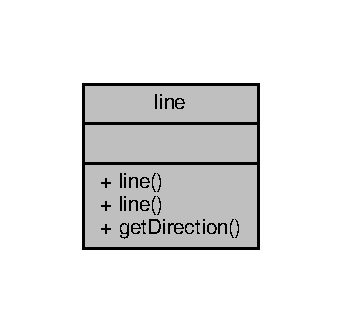
\includegraphics[width=164pt]{classline__coll__graph}
\end{center}
\end{figure}
\subsection*{Public Member Functions}
\begin{DoxyCompactItemize}
\item 
\mbox{\hyperlink{classline_af35f570d03c98b54683f8d0df5e376dc}{line}} (\mbox{\hyperlink{classpoint}{point}} p1, \mbox{\hyperlink{classpoint}{point}} p2)
\item 
\mbox{\hyperlink{classline_a5c7c332f2c5e4badc9bdfa807b4aef86}{line}} (float a, float b, float c)
\item 
\mbox{\hyperlink{classpoint}{point}} \mbox{\hyperlink{classline_a72da40e3a2e2efaa58ee7a379415b2c5}{get\+Direction}} ()
\end{DoxyCompactItemize}


\subsection{Constructor \& Destructor Documentation}
\mbox{\Hypertarget{classline_af35f570d03c98b54683f8d0df5e376dc}\label{classline_af35f570d03c98b54683f8d0df5e376dc}} 
\index{line@{line}!line@{line}}
\index{line@{line}!line@{line}}
\subsubsection{\texorpdfstring{line()}{line()}\hspace{0.1cm}{\footnotesize\ttfamily [1/2]}}
{\footnotesize\ttfamily line\+::line (\begin{DoxyParamCaption}\item[{\mbox{\hyperlink{classpoint}{point}}}]{p1,  }\item[{\mbox{\hyperlink{classpoint}{point}}}]{p2 }\end{DoxyParamCaption})}

\mbox{\Hypertarget{classline_a5c7c332f2c5e4badc9bdfa807b4aef86}\label{classline_a5c7c332f2c5e4badc9bdfa807b4aef86}} 
\index{line@{line}!line@{line}}
\index{line@{line}!line@{line}}
\subsubsection{\texorpdfstring{line()}{line()}\hspace{0.1cm}{\footnotesize\ttfamily [2/2]}}
{\footnotesize\ttfamily line\+::line (\begin{DoxyParamCaption}\item[{float}]{a,  }\item[{float}]{b,  }\item[{float}]{c }\end{DoxyParamCaption})}



\subsection{Member Function Documentation}
\mbox{\Hypertarget{classline_a72da40e3a2e2efaa58ee7a379415b2c5}\label{classline_a72da40e3a2e2efaa58ee7a379415b2c5}} 
\index{line@{line}!get\+Direction@{get\+Direction}}
\index{get\+Direction@{get\+Direction}!line@{line}}
\subsubsection{\texorpdfstring{get\+Direction()}{getDirection()}}
{\footnotesize\ttfamily \mbox{\hyperlink{classpoint}{point}} line\+::get\+Direction (\begin{DoxyParamCaption}{ }\end{DoxyParamCaption})}

\begin{DoxyReturn}{Returns}
direction pointed to by the line 
\end{DoxyReturn}


The documentation for this class was generated from the following file\+:\begin{DoxyCompactItemize}
\item 
\mbox{\hyperlink{point_8h}{point.\+h}}\end{DoxyCompactItemize}

\hypertarget{classobject2D}{}\section{object2D Class Reference}
\label{classobject2D}\index{object2D@{object2D}}


{\ttfamily \#include $<$object2\+D.\+h$>$}



Collaboration diagram for object2D\+:
\nopagebreak
\begin{figure}[H]
\begin{center}
\leavevmode
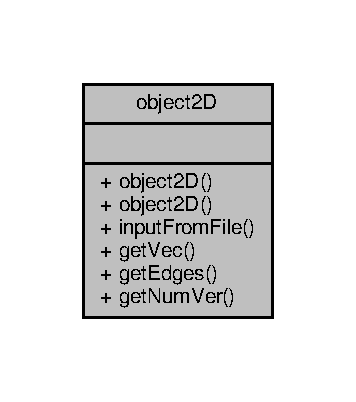
\includegraphics[width=171pt]{classobject2D__coll__graph}
\end{center}
\end{figure}
\subsection*{Public Member Functions}
\begin{DoxyCompactItemize}
\item 
\mbox{\hyperlink{classobject2D_a2169d77e7375f31356d2524c26c0a63f}{object2D}} ()
\item 
\mbox{\hyperlink{classobject2D_a7c2dd1d0bae14f68311ffa3194c7b848}{object2D}} (vector$<$ glm\+::vec4 $>$ vertices\+\_\+vec\+\_\+2d, vector$<$ vector$<$ int $>$ $>$ line\+\_\+2d)
\item 
void \mbox{\hyperlink{classobject2D_a6697aecc21bb2348fb81950cc0d83c83}{input\+From\+File}} (string filename)
\item 
vector$<$ glm\+::vec4 $>$ \mbox{\hyperlink{classobject2D_a529cdc088990e491fef49b97f58c9a5a}{get\+Vec}} ()
\item 
vector$<$ vector$<$ int $>$ $>$ \mbox{\hyperlink{classobject2D_a22bb00cbc061128b26645e6cdf7a2117}{get\+Edges}} ()
\item 
int \mbox{\hyperlink{classobject2D_a957470b9b7c66bf1def476cd4b7d5fde}{get\+Num\+Ver}} ()
\end{DoxyCompactItemize}


\subsection{Constructor \& Destructor Documentation}
\mbox{\Hypertarget{classobject2D_a2169d77e7375f31356d2524c26c0a63f}\label{classobject2D_a2169d77e7375f31356d2524c26c0a63f}} 
\index{object2D@{object2D}!object2D@{object2D}}
\index{object2D@{object2D}!object2D@{object2D}}
\subsubsection{\texorpdfstring{object2\+D()}{object2D()}\hspace{0.1cm}{\footnotesize\ttfamily [1/2]}}
{\footnotesize\ttfamily object2\+D\+::object2D (\begin{DoxyParamCaption}{ }\end{DoxyParamCaption})}

constructor for the 2D figure class \mbox{\Hypertarget{classobject2D_a7c2dd1d0bae14f68311ffa3194c7b848}\label{classobject2D_a7c2dd1d0bae14f68311ffa3194c7b848}} 
\index{object2D@{object2D}!object2D@{object2D}}
\index{object2D@{object2D}!object2D@{object2D}}
\subsubsection{\texorpdfstring{object2\+D()}{object2D()}\hspace{0.1cm}{\footnotesize\ttfamily [2/2]}}
{\footnotesize\ttfamily object2\+D\+::object2D (\begin{DoxyParamCaption}\item[{vector$<$ glm\+::vec4 $>$}]{vertices\+\_\+vec\+\_\+2d,  }\item[{vector$<$ vector$<$ int $>$ $>$}]{line\+\_\+2d }\end{DoxyParamCaption})}



\subsection{Member Function Documentation}
\mbox{\Hypertarget{classobject2D_a22bb00cbc061128b26645e6cdf7a2117}\label{classobject2D_a22bb00cbc061128b26645e6cdf7a2117}} 
\index{object2D@{object2D}!get\+Edges@{get\+Edges}}
\index{get\+Edges@{get\+Edges}!object2D@{object2D}}
\subsubsection{\texorpdfstring{get\+Edges()}{getEdges()}}
{\footnotesize\ttfamily vector$<$vector$<$int$>$ $>$ object2\+D\+::get\+Edges (\begin{DoxyParamCaption}{ }\end{DoxyParamCaption})}

function to return the edges between all the vertices of the object in form of adjacency list. \mbox{\Hypertarget{classobject2D_a957470b9b7c66bf1def476cd4b7d5fde}\label{classobject2D_a957470b9b7c66bf1def476cd4b7d5fde}} 
\index{object2D@{object2D}!get\+Num\+Ver@{get\+Num\+Ver}}
\index{get\+Num\+Ver@{get\+Num\+Ver}!object2D@{object2D}}
\subsubsection{\texorpdfstring{get\+Num\+Ver()}{getNumVer()}}
{\footnotesize\ttfamily int object2\+D\+::get\+Num\+Ver (\begin{DoxyParamCaption}{ }\end{DoxyParamCaption})}

function to return the number of vertices in the object. \mbox{\Hypertarget{classobject2D_a529cdc088990e491fef49b97f58c9a5a}\label{classobject2D_a529cdc088990e491fef49b97f58c9a5a}} 
\index{object2D@{object2D}!get\+Vec@{get\+Vec}}
\index{get\+Vec@{get\+Vec}!object2D@{object2D}}
\subsubsection{\texorpdfstring{get\+Vec()}{getVec()}}
{\footnotesize\ttfamily vector$<$glm\+::vec4$>$ object2\+D\+::get\+Vec (\begin{DoxyParamCaption}{ }\end{DoxyParamCaption})}

function to return all the coordinates of the 2d object \mbox{\Hypertarget{classobject2D_a6697aecc21bb2348fb81950cc0d83c83}\label{classobject2D_a6697aecc21bb2348fb81950cc0d83c83}} 
\index{object2D@{object2D}!input\+From\+File@{input\+From\+File}}
\index{input\+From\+File@{input\+From\+File}!object2D@{object2D}}
\subsubsection{\texorpdfstring{input\+From\+File()}{inputFromFile()}}
{\footnotesize\ttfamily void object2\+D\+::input\+From\+File (\begin{DoxyParamCaption}\item[{string}]{filename }\end{DoxyParamCaption})}

function to input the 2D figure from file 
\begin{DoxyParams}{Parameters}
{\em filename} & File to be taken as input Then it check the consistency If inconsistant, raises exception else constructs the object \\
\hline
\end{DoxyParams}


The documentation for this class was generated from the following file\+:\begin{DoxyCompactItemize}
\item 
\mbox{\hyperlink{object2D_8h}{object2\+D.\+h}}\end{DoxyCompactItemize}

\hypertarget{classobject3D}{}\section{object3D Class Reference}
\label{classobject3D}\index{object3D@{object3D}}


{\ttfamily \#include $<$object3\+D.\+h$>$}



Collaboration diagram for object3D\+:
\nopagebreak
\begin{figure}[H]
\begin{center}
\leavevmode
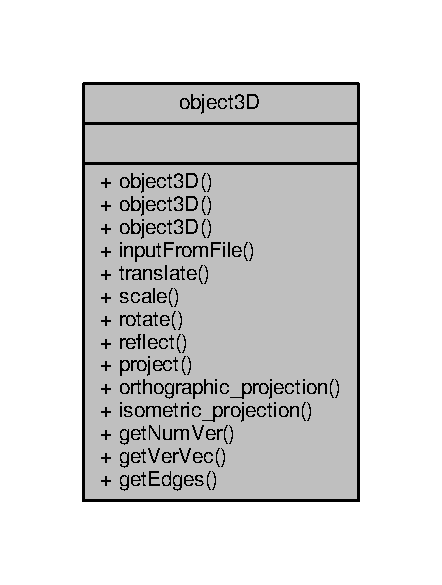
\includegraphics[width=212pt]{classobject3D__coll__graph}
\end{center}
\end{figure}
\subsection*{Public Member Functions}
\begin{DoxyCompactItemize}
\item 
\mbox{\hyperlink{classobject3D_a0911667d0108c1ae15a60a3e120a2a73}{object3D}} ()
\item 
\mbox{\hyperlink{classobject3D_a1c60c123d02bd02d9ca35fd507fb81cd}{object3D}} (vector$<$ glm\+::vec4 $>$ vertices\+\_\+vec\+\_\+3d, vector$<$ vector$<$ int $>$ $>$ line\+\_\+3d)
\item 
\mbox{\hyperlink{classobject3D_a6837b926d352b2fd1aff01bed902f1bf}{object3D}} (\mbox{\hyperlink{classorthographic}{orthographic}} obj)
\item 
void \mbox{\hyperlink{classobject3D_ab9f47d0de463217dd4cc816d16bf1661}{input\+From\+File}} (string filename)
\item 
void \mbox{\hyperlink{classobject3D_a78772ee3fafc1ad79168776baef859fa}{translate}} (float x=0.\+0, float y=0.\+0, float z=0.\+0)
\item 
void \mbox{\hyperlink{classobject3D_ab12153ab6a9092e85db7912670d55a48}{scale}} (float x=1.\+0, float y=1.\+0, float z=1.\+0)
\item 
void \mbox{\hyperlink{classobject3D_a9599c3e6c9ea35b9496d4b5b14623b5b}{rotate}} (float theta, \mbox{\hyperlink{classline}{line}} axis)
\item 
void \mbox{\hyperlink{classobject3D_a63af641d18acc59e4ff0cae8387b06bc}{reflect}} (\mbox{\hyperlink{classplane}{plane}} p)
\item 
\mbox{\hyperlink{classobject2D}{object2D}} \mbox{\hyperlink{classobject3D_a4b7bdf9d5a609b34e1ca22490538a37d}{project}} (\mbox{\hyperlink{classplane}{plane}} p)
\item 
\mbox{\hyperlink{classorthographic}{orthographic}} \mbox{\hyperlink{classobject3D_a7bb948cdf51a8143338bb8a22e97f910}{orthographic\+\_\+projection}} ()
\item 
\mbox{\hyperlink{classobject2D}{object2D}} \mbox{\hyperlink{classobject3D_a18f7b37e4d847917835205c9faf0885e}{isometric\+\_\+projection}} ()
\item 
int \mbox{\hyperlink{classobject3D_aeb34ac3e26a3c7a8190f2abadfaa370a}{get\+Num\+Ver}} ()
\item 
vector$<$ glm\+::vec4 $>$ \mbox{\hyperlink{classobject3D_a9b0407c5b8444f840d3bebaf3deac07f}{get\+Ver\+Vec}} ()
\item 
vector$<$ vector$<$ int $>$ $>$ \mbox{\hyperlink{classobject3D_a4ed285050b7a9def183cbba66766934d}{get\+Edges}} ()
\end{DoxyCompactItemize}


\subsection{Constructor \& Destructor Documentation}
\mbox{\Hypertarget{classobject3D_a0911667d0108c1ae15a60a3e120a2a73}\label{classobject3D_a0911667d0108c1ae15a60a3e120a2a73}} 
\index{object3D@{object3D}!object3D@{object3D}}
\index{object3D@{object3D}!object3D@{object3D}}
\subsubsection{\texorpdfstring{object3\+D()}{object3D()}\hspace{0.1cm}{\footnotesize\ttfamily [1/3]}}
{\footnotesize\ttfamily object3\+D\+::object3D (\begin{DoxyParamCaption}{ }\end{DoxyParamCaption})}

Constructs a blank 3D figure \mbox{\Hypertarget{classobject3D_a1c60c123d02bd02d9ca35fd507fb81cd}\label{classobject3D_a1c60c123d02bd02d9ca35fd507fb81cd}} 
\index{object3D@{object3D}!object3D@{object3D}}
\index{object3D@{object3D}!object3D@{object3D}}
\subsubsection{\texorpdfstring{object3\+D()}{object3D()}\hspace{0.1cm}{\footnotesize\ttfamily [2/3]}}
{\footnotesize\ttfamily object3\+D\+::object3D (\begin{DoxyParamCaption}\item[{vector$<$ glm\+::vec4 $>$}]{vertices\+\_\+vec\+\_\+3d,  }\item[{vector$<$ vector$<$ int $>$ $>$}]{line\+\_\+3d }\end{DoxyParamCaption})}

contructor of \mbox{\hyperlink{classobject3D}{object3D}} class given the vertices coordinates and the connection of points stored in adjacency list. 
\begin{DoxyParams}{Parameters}
{\em vertices\+\_\+vec\+\_\+3d} & vertices co-\/ordinates \\
\hline
{\em line\+\_\+3d} & adjacency list of connection of points. \\
\hline
\end{DoxyParams}
\mbox{\Hypertarget{classobject3D_a6837b926d352b2fd1aff01bed902f1bf}\label{classobject3D_a6837b926d352b2fd1aff01bed902f1bf}} 
\index{object3D@{object3D}!object3D@{object3D}}
\index{object3D@{object3D}!object3D@{object3D}}
\subsubsection{\texorpdfstring{object3\+D()}{object3D()}\hspace{0.1cm}{\footnotesize\ttfamily [3/3]}}
{\footnotesize\ttfamily object3\+D\+::object3D (\begin{DoxyParamCaption}\item[{\mbox{\hyperlink{classorthographic}{orthographic}}}]{obj }\end{DoxyParamCaption})}

Function to interactively input the points and their connections in form of lines and then it check the consistency If inconsistent, raises exception else constructs the object. 

\subsection{Member Function Documentation}
\mbox{\Hypertarget{classobject3D_a4ed285050b7a9def183cbba66766934d}\label{classobject3D_a4ed285050b7a9def183cbba66766934d}} 
\index{object3D@{object3D}!get\+Edges@{get\+Edges}}
\index{get\+Edges@{get\+Edges}!object3D@{object3D}}
\subsubsection{\texorpdfstring{get\+Edges()}{getEdges()}}
{\footnotesize\ttfamily vector$<$vector$<$int$>$ $>$ object3\+D\+::get\+Edges (\begin{DoxyParamCaption}{ }\end{DoxyParamCaption})}

function to return the edges between all the vertices of the object in form of adjacency list. \mbox{\Hypertarget{classobject3D_aeb34ac3e26a3c7a8190f2abadfaa370a}\label{classobject3D_aeb34ac3e26a3c7a8190f2abadfaa370a}} 
\index{object3D@{object3D}!get\+Num\+Ver@{get\+Num\+Ver}}
\index{get\+Num\+Ver@{get\+Num\+Ver}!object3D@{object3D}}
\subsubsection{\texorpdfstring{get\+Num\+Ver()}{getNumVer()}}
{\footnotesize\ttfamily int object3\+D\+::get\+Num\+Ver (\begin{DoxyParamCaption}{ }\end{DoxyParamCaption})}

function to return the number of vertices in the object. \mbox{\Hypertarget{classobject3D_a9b0407c5b8444f840d3bebaf3deac07f}\label{classobject3D_a9b0407c5b8444f840d3bebaf3deac07f}} 
\index{object3D@{object3D}!get\+Ver\+Vec@{get\+Ver\+Vec}}
\index{get\+Ver\+Vec@{get\+Ver\+Vec}!object3D@{object3D}}
\subsubsection{\texorpdfstring{get\+Ver\+Vec()}{getVerVec()}}
{\footnotesize\ttfamily vector$<$glm\+::vec4$>$ object3\+D\+::get\+Ver\+Vec (\begin{DoxyParamCaption}{ }\end{DoxyParamCaption})}

function to return all the coordinates of the 2d object \mbox{\Hypertarget{classobject3D_ab9f47d0de463217dd4cc816d16bf1661}\label{classobject3D_ab9f47d0de463217dd4cc816d16bf1661}} 
\index{object3D@{object3D}!input\+From\+File@{input\+From\+File}}
\index{input\+From\+File@{input\+From\+File}!object3D@{object3D}}
\subsubsection{\texorpdfstring{input\+From\+File()}{inputFromFile()}}
{\footnotesize\ttfamily void object3\+D\+::input\+From\+File (\begin{DoxyParamCaption}\item[{string}]{filename }\end{DoxyParamCaption})}

Function to input the 2D figure from file and then it check the consistency If inconsistent, raises exception else constructs the object. 
\begin{DoxyParams}{Parameters}
{\em filename} & File to be taken as input \\
\hline
\end{DoxyParams}
\mbox{\Hypertarget{classobject3D_a18f7b37e4d847917835205c9faf0885e}\label{classobject3D_a18f7b37e4d847917835205c9faf0885e}} 
\index{object3D@{object3D}!isometric\+\_\+projection@{isometric\+\_\+projection}}
\index{isometric\+\_\+projection@{isometric\+\_\+projection}!object3D@{object3D}}
\subsubsection{\texorpdfstring{isometric\+\_\+projection()}{isometric\_projection()}}
{\footnotesize\ttfamily \mbox{\hyperlink{classobject2D}{object2D}} object3\+D\+::isometric\+\_\+projection (\begin{DoxyParamCaption}{ }\end{DoxyParamCaption})}

Calculates isometric projection of the 3D Figure \mbox{\Hypertarget{classobject3D_a7bb948cdf51a8143338bb8a22e97f910}\label{classobject3D_a7bb948cdf51a8143338bb8a22e97f910}} 
\index{object3D@{object3D}!orthographic\+\_\+projection@{orthographic\+\_\+projection}}
\index{orthographic\+\_\+projection@{orthographic\+\_\+projection}!object3D@{object3D}}
\subsubsection{\texorpdfstring{orthographic\+\_\+projection()}{orthographic\_projection()}}
{\footnotesize\ttfamily \mbox{\hyperlink{classorthographic}{orthographic}} object3\+D\+::orthographic\+\_\+projection (\begin{DoxyParamCaption}{ }\end{DoxyParamCaption})}

Calculates orthographic projections of the 3D Figure \mbox{\Hypertarget{classobject3D_a4b7bdf9d5a609b34e1ca22490538a37d}\label{classobject3D_a4b7bdf9d5a609b34e1ca22490538a37d}} 
\index{object3D@{object3D}!project@{project}}
\index{project@{project}!object3D@{object3D}}
\subsubsection{\texorpdfstring{project()}{project()}}
{\footnotesize\ttfamily \mbox{\hyperlink{classobject2D}{object2D}} object3\+D\+::project (\begin{DoxyParamCaption}\item[{\mbox{\hyperlink{classplane}{plane}}}]{p }\end{DoxyParamCaption})}

Projects the 3D Figure on a given plane 
\begin{DoxyParams}{Parameters}
{\em p} & plane on which to project \\
\hline
\end{DoxyParams}
\mbox{\Hypertarget{classobject3D_a63af641d18acc59e4ff0cae8387b06bc}\label{classobject3D_a63af641d18acc59e4ff0cae8387b06bc}} 
\index{object3D@{object3D}!reflect@{reflect}}
\index{reflect@{reflect}!object3D@{object3D}}
\subsubsection{\texorpdfstring{reflect()}{reflect()}}
{\footnotesize\ttfamily void object3\+D\+::reflect (\begin{DoxyParamCaption}\item[{\mbox{\hyperlink{classplane}{plane}}}]{p }\end{DoxyParamCaption})}

Reflects an object about a given plane 
\begin{DoxyParams}{Parameters}
{\em p} & plane about which to reflect \\
\hline
\end{DoxyParams}
\mbox{\Hypertarget{classobject3D_a9599c3e6c9ea35b9496d4b5b14623b5b}\label{classobject3D_a9599c3e6c9ea35b9496d4b5b14623b5b}} 
\index{object3D@{object3D}!rotate@{rotate}}
\index{rotate@{rotate}!object3D@{object3D}}
\subsubsection{\texorpdfstring{rotate()}{rotate()}}
{\footnotesize\ttfamily void object3\+D\+::rotate (\begin{DoxyParamCaption}\item[{float}]{theta,  }\item[{\mbox{\hyperlink{classline}{line}}}]{axis }\end{DoxyParamCaption})}

Rotates the figure around a given axis by a given angle 
\begin{DoxyParams}{Parameters}
{\em theta} & angle to be rotated by \\
\hline
{\em axis} & axis about which object is to be rotated \\
\hline
\end{DoxyParams}
\mbox{\Hypertarget{classobject3D_ab12153ab6a9092e85db7912670d55a48}\label{classobject3D_ab12153ab6a9092e85db7912670d55a48}} 
\index{object3D@{object3D}!scale@{scale}}
\index{scale@{scale}!object3D@{object3D}}
\subsubsection{\texorpdfstring{scale()}{scale()}}
{\footnotesize\ttfamily void object3\+D\+::scale (\begin{DoxyParamCaption}\item[{float}]{x = {\ttfamily 1.0},  }\item[{float}]{y = {\ttfamily 1.0},  }\item[{float}]{z = {\ttfamily 1.0} }\end{DoxyParamCaption})}

Scales the 3D Figure proportionately 
\begin{DoxyParams}{Parameters}
{\em x} & amount of scaling in x-\/direction \\
\hline
{\em y} & amount of scaling in y-\/direction \\
\hline
{\em z} & amount of scaling in z-\/direction \\
\hline
\end{DoxyParams}
\mbox{\Hypertarget{classobject3D_a78772ee3fafc1ad79168776baef859fa}\label{classobject3D_a78772ee3fafc1ad79168776baef859fa}} 
\index{object3D@{object3D}!translate@{translate}}
\index{translate@{translate}!object3D@{object3D}}
\subsubsection{\texorpdfstring{translate()}{translate()}}
{\footnotesize\ttfamily void object3\+D\+::translate (\begin{DoxyParamCaption}\item[{float}]{x = {\ttfamily 0.0},  }\item[{float}]{y = {\ttfamily 0.0},  }\item[{float}]{z = {\ttfamily 0.0} }\end{DoxyParamCaption})}

Translates the 3D Figure to a different 3D location. 
\begin{DoxyParams}{Parameters}
{\em x} & amount of translation in x-\/direction \\
\hline
{\em y} & amount of translation in y-\/direction \\
\hline
{\em z} & amount of translation in z-\/direction \\
\hline
\end{DoxyParams}


The documentation for this class was generated from the following file\+:\begin{DoxyCompactItemize}
\item 
\mbox{\hyperlink{object3D_8h}{object3\+D.\+h}}\end{DoxyCompactItemize}

\hypertarget{classorthographic}{}\section{orthographic Class Reference}
\label{classorthographic}\index{orthographic@{orthographic}}


{\ttfamily \#include $<$orthographic.\+h$>$}



Collaboration diagram for orthographic\+:
\nopagebreak
\begin{figure}[H]
\begin{center}
\leavevmode
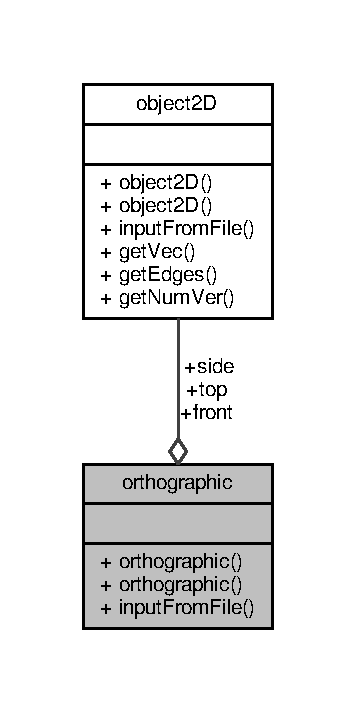
\includegraphics[width=171pt]{classorthographic__coll__graph}
\end{center}
\end{figure}
\subsection*{Public Member Functions}
\begin{DoxyCompactItemize}
\item 
\mbox{\hyperlink{classorthographic_a6f77ed4c0885e17bd4fbb8514338f62e}{orthographic}} (\mbox{\hyperlink{classobject2D}{object2D}} f, \mbox{\hyperlink{classobject2D}{object2D}} s, \mbox{\hyperlink{classobject2D}{object2D}} t)
\item 
\mbox{\hyperlink{classorthographic_ac461c4656ab5617ff11f091663355869}{orthographic}} ()
\item 
void \mbox{\hyperlink{classorthographic_a0d8e45328b99b53d243bffc5f5d795b6}{input\+From\+File}} (string filename)
\end{DoxyCompactItemize}
\subsection*{Public Attributes}
\begin{DoxyCompactItemize}
\item 
\mbox{\hyperlink{classobject2D}{object2D}} \mbox{\hyperlink{classorthographic_a4612638f537edd8d23c95061669a2599}{front}}
\item 
\mbox{\hyperlink{classobject2D}{object2D}} \mbox{\hyperlink{classorthographic_a37d0964ad1151feda26b3c9498b1075b}{side}}
\item 
\mbox{\hyperlink{classobject2D}{object2D}} \mbox{\hyperlink{classorthographic_ac0978ff6a9a243e3d8ed21efffe041b4}{top}}
\end{DoxyCompactItemize}


\subsection{Constructor \& Destructor Documentation}
\mbox{\Hypertarget{classorthographic_a6f77ed4c0885e17bd4fbb8514338f62e}\label{classorthographic_a6f77ed4c0885e17bd4fbb8514338f62e}} 
\index{orthographic@{orthographic}!orthographic@{orthographic}}
\index{orthographic@{orthographic}!orthographic@{orthographic}}
\subsubsection{\texorpdfstring{orthographic()}{orthographic()}\hspace{0.1cm}{\footnotesize\ttfamily [1/2]}}
{\footnotesize\ttfamily orthographic\+::orthographic (\begin{DoxyParamCaption}\item[{\mbox{\hyperlink{classobject2D}{object2D}}}]{f,  }\item[{\mbox{\hyperlink{classobject2D}{object2D}}}]{s,  }\item[{\mbox{\hyperlink{classobject2D}{object2D}}}]{t }\end{DoxyParamCaption})}

constructor of the orthographic views 
\begin{DoxyParams}{Parameters}
{\em f} & Takes the reference of the front view 2D object \\
\hline
{\em ba} & Takes the reference of the back view 2D object \\
\hline
{\em l} & Takes the reference of the left view 2D object \\
\hline
{\em r} & Takes the reference of the right view 2D object \\
\hline
{\em t} & Takes the reference of the top view 2D object \\
\hline
{\em bo} & Takes the reference of the bottom view 2D object \\
\hline
\end{DoxyParams}
\mbox{\Hypertarget{classorthographic_ac461c4656ab5617ff11f091663355869}\label{classorthographic_ac461c4656ab5617ff11f091663355869}} 
\index{orthographic@{orthographic}!orthographic@{orthographic}}
\index{orthographic@{orthographic}!orthographic@{orthographic}}
\subsubsection{\texorpdfstring{orthographic()}{orthographic()}\hspace{0.1cm}{\footnotesize\ttfamily [2/2]}}
{\footnotesize\ttfamily orthographic\+::orthographic (\begin{DoxyParamCaption}{ }\end{DoxyParamCaption})}



\subsection{Member Function Documentation}
\mbox{\Hypertarget{classorthographic_a0d8e45328b99b53d243bffc5f5d795b6}\label{classorthographic_a0d8e45328b99b53d243bffc5f5d795b6}} 
\index{orthographic@{orthographic}!input\+From\+File@{input\+From\+File}}
\index{input\+From\+File@{input\+From\+File}!orthographic@{orthographic}}
\subsubsection{\texorpdfstring{input\+From\+File()}{inputFromFile()}}
{\footnotesize\ttfamily void orthographic\+::input\+From\+File (\begin{DoxyParamCaption}\item[{string}]{filename }\end{DoxyParamCaption})}


\begin{DoxyParams}{Parameters}
{\em filename} & File from which input is taken. \\
\hline
\end{DoxyParams}


\subsection{Member Data Documentation}
\mbox{\Hypertarget{classorthographic_a4612638f537edd8d23c95061669a2599}\label{classorthographic_a4612638f537edd8d23c95061669a2599}} 
\index{orthographic@{orthographic}!front@{front}}
\index{front@{front}!orthographic@{orthographic}}
\subsubsection{\texorpdfstring{front}{front}}
{\footnotesize\ttfamily \mbox{\hyperlink{classobject2D}{object2D}} orthographic\+::front}

\mbox{\Hypertarget{classorthographic_a37d0964ad1151feda26b3c9498b1075b}\label{classorthographic_a37d0964ad1151feda26b3c9498b1075b}} 
\index{orthographic@{orthographic}!side@{side}}
\index{side@{side}!orthographic@{orthographic}}
\subsubsection{\texorpdfstring{side}{side}}
{\footnotesize\ttfamily \mbox{\hyperlink{classobject2D}{object2D}} orthographic\+::side}

\mbox{\Hypertarget{classorthographic_ac0978ff6a9a243e3d8ed21efffe041b4}\label{classorthographic_ac0978ff6a9a243e3d8ed21efffe041b4}} 
\index{orthographic@{orthographic}!top@{top}}
\index{top@{top}!orthographic@{orthographic}}
\subsubsection{\texorpdfstring{top}{top}}
{\footnotesize\ttfamily \mbox{\hyperlink{classobject2D}{object2D}} orthographic\+::top}



The documentation for this class was generated from the following file\+:\begin{DoxyCompactItemize}
\item 
\mbox{\hyperlink{orthographic_8h}{orthographic.\+h}}\end{DoxyCompactItemize}

\hypertarget{classplane}{}\section{plane Class Reference}
\label{classplane}\index{plane@{plane}}


{\ttfamily \#include $<$point.\+h$>$}



Collaboration diagram for plane\+:\nopagebreak
\begin{figure}[H]
\begin{center}
\leavevmode
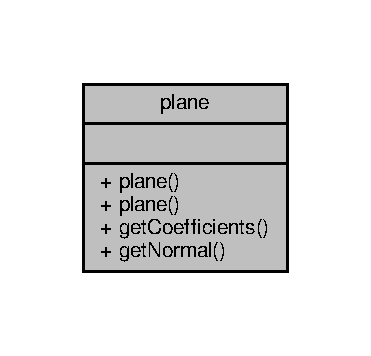
\includegraphics[width=178pt]{classplane__coll__graph}
\end{center}
\end{figure}
\subsection*{Public Member Functions}
\begin{DoxyCompactItemize}
\item 
\mbox{\hyperlink{classplane_ac97881e6c8bdc9adaaf1db251b68d485}{plane}} (float A, float B, float C, float D)
\item 
\mbox{\hyperlink{classplane_a63d7a83ca8a345da5ee6de3c67b8de0c}{plane}} (\mbox{\hyperlink{classpoint}{point}} p, \mbox{\hyperlink{classline}{line}} nor)
\item 
float $\ast$ \mbox{\hyperlink{classplane_af4424e6ded2a9c57af4793aea84f56d2}{get\+Coefficients}} ()
\item 
\mbox{\hyperlink{classpoint}{point}} \mbox{\hyperlink{classplane_a4de93e2552aa7be05807f234dd02fbda}{get\+Normal}} ()
\end{DoxyCompactItemize}


\subsection{Constructor \& Destructor Documentation}
\mbox{\Hypertarget{classplane_ac97881e6c8bdc9adaaf1db251b68d485}\label{classplane_ac97881e6c8bdc9adaaf1db251b68d485}} 
\index{plane@{plane}!plane@{plane}}
\index{plane@{plane}!plane@{plane}}
\subsubsection{\texorpdfstring{plane()}{plane()}\hspace{0.1cm}{\footnotesize\ttfamily [1/2]}}
{\footnotesize\ttfamily plane\+::plane (\begin{DoxyParamCaption}\item[{float}]{A,  }\item[{float}]{B,  }\item[{float}]{C,  }\item[{float}]{D }\end{DoxyParamCaption})}

\mbox{\Hypertarget{classplane_a63d7a83ca8a345da5ee6de3c67b8de0c}\label{classplane_a63d7a83ca8a345da5ee6de3c67b8de0c}} 
\index{plane@{plane}!plane@{plane}}
\index{plane@{plane}!plane@{plane}}
\subsubsection{\texorpdfstring{plane()}{plane()}\hspace{0.1cm}{\footnotesize\ttfamily [2/2]}}
{\footnotesize\ttfamily plane\+::plane (\begin{DoxyParamCaption}\item[{\mbox{\hyperlink{classpoint}{point}}}]{p,  }\item[{\mbox{\hyperlink{classline}{line}}}]{nor }\end{DoxyParamCaption})}



\subsection{Member Function Documentation}
\mbox{\Hypertarget{classplane_af4424e6ded2a9c57af4793aea84f56d2}\label{classplane_af4424e6ded2a9c57af4793aea84f56d2}} 
\index{plane@{plane}!get\+Coefficients@{get\+Coefficients}}
\index{get\+Coefficients@{get\+Coefficients}!plane@{plane}}
\subsubsection{\texorpdfstring{get\+Coefficients()}{getCoefficients()}}
{\footnotesize\ttfamily float$\ast$ plane\+::get\+Coefficients (\begin{DoxyParamCaption}{ }\end{DoxyParamCaption})}

Returns an array containing the co-\/efficients of the plane a,b,c,d respectively \mbox{\Hypertarget{classplane_a4de93e2552aa7be05807f234dd02fbda}\label{classplane_a4de93e2552aa7be05807f234dd02fbda}} 
\index{plane@{plane}!get\+Normal@{get\+Normal}}
\index{get\+Normal@{get\+Normal}!plane@{plane}}
\subsubsection{\texorpdfstring{get\+Normal()}{getNormal()}}
{\footnotesize\ttfamily \mbox{\hyperlink{classpoint}{point}} plane\+::get\+Normal (\begin{DoxyParamCaption}{ }\end{DoxyParamCaption})}

Returns the normal of the plane \begin{DoxyReturn}{Returns}
A vector representing the components along x, y, and z directions 
\end{DoxyReturn}


The documentation for this class was generated from the following file\+:\begin{DoxyCompactItemize}
\item 
\mbox{\hyperlink{point_8h}{point.\+h}}\end{DoxyCompactItemize}

\hypertarget{classpoint}{}\section{point Class Reference}
\label{classpoint}\index{point@{point}}


{\ttfamily \#include $<$point.\+h$>$}



Collaboration diagram for point\+:\nopagebreak
\begin{figure}[H]
\begin{center}
\leavevmode
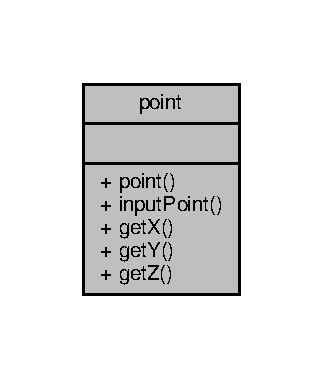
\includegraphics[width=155pt]{classpoint__coll__graph}
\end{center}
\end{figure}
\subsection*{Public Member Functions}
\begin{DoxyCompactItemize}
\item 
\mbox{\hyperlink{classpoint_a390f735b876631979040ab611bdf36cb}{point}} (float x\+\_\+coord, float y\+\_\+coord, float z\+\_\+coord)
\item 
void \mbox{\hyperlink{classpoint_a91fdb8a1d1dded9dba1a3dc648d94c84}{input\+Point}} ()
\item 
float \mbox{\hyperlink{classpoint_a6cafeeff09ea34a0aac36273373b5814}{getX}} ()
\item 
float \mbox{\hyperlink{classpoint_ac5d9deb8d3dc8f0c64a1fa8d612b44f4}{getY}} ()
\item 
float \mbox{\hyperlink{classpoint_a18aa4ec7b86492b7c2af4d92a0d09a57}{getZ}} ()
\end{DoxyCompactItemize}


\subsection{Constructor \& Destructor Documentation}
\mbox{\Hypertarget{classpoint_a390f735b876631979040ab611bdf36cb}\label{classpoint_a390f735b876631979040ab611bdf36cb}} 
\index{point@{point}!point@{point}}
\index{point@{point}!point@{point}}
\subsubsection{\texorpdfstring{point()}{point()}}
{\footnotesize\ttfamily point\+::point (\begin{DoxyParamCaption}\item[{float}]{x\+\_\+coord,  }\item[{float}]{y\+\_\+coord,  }\item[{float}]{z\+\_\+coord }\end{DoxyParamCaption})}

class to store the point for the graphics object 
\begin{DoxyParams}{Parameters}
{\em x\+\_\+coord} & X-\/coordinate with default initilisation zero \\
\hline
{\em y\+\_\+coord} & Y-\/coordinate with default initilisation zero \\
\hline
{\em z\+\_\+coord} & Z-\/coordinate with default initilisation zero \\
\hline
\end{DoxyParams}


\subsection{Member Function Documentation}
\mbox{\Hypertarget{classpoint_a6cafeeff09ea34a0aac36273373b5814}\label{classpoint_a6cafeeff09ea34a0aac36273373b5814}} 
\index{point@{point}!getX@{getX}}
\index{getX@{getX}!point@{point}}
\subsubsection{\texorpdfstring{get\+X()}{getX()}}
{\footnotesize\ttfamily float point\+::getX (\begin{DoxyParamCaption}{ }\end{DoxyParamCaption})}

returns the x-\/coordinate of the point \mbox{\Hypertarget{classpoint_ac5d9deb8d3dc8f0c64a1fa8d612b44f4}\label{classpoint_ac5d9deb8d3dc8f0c64a1fa8d612b44f4}} 
\index{point@{point}!getY@{getY}}
\index{getY@{getY}!point@{point}}
\subsubsection{\texorpdfstring{get\+Y()}{getY()}}
{\footnotesize\ttfamily float point\+::getY (\begin{DoxyParamCaption}{ }\end{DoxyParamCaption})}

returns the y-\/coordinate of the point \mbox{\Hypertarget{classpoint_a18aa4ec7b86492b7c2af4d92a0d09a57}\label{classpoint_a18aa4ec7b86492b7c2af4d92a0d09a57}} 
\index{point@{point}!getZ@{getZ}}
\index{getZ@{getZ}!point@{point}}
\subsubsection{\texorpdfstring{get\+Z()}{getZ()}}
{\footnotesize\ttfamily float point\+::getZ (\begin{DoxyParamCaption}{ }\end{DoxyParamCaption})}

returns the z-\/coordinate of the point \mbox{\Hypertarget{classpoint_a91fdb8a1d1dded9dba1a3dc648d94c84}\label{classpoint_a91fdb8a1d1dded9dba1a3dc648d94c84}} 
\index{point@{point}!input\+Point@{input\+Point}}
\index{input\+Point@{input\+Point}!point@{point}}
\subsubsection{\texorpdfstring{input\+Point()}{inputPoint()}}
{\footnotesize\ttfamily void point\+::input\+Point (\begin{DoxyParamCaption}{ }\end{DoxyParamCaption})}

input the x,y,z coordinate in that order from stdin 

The documentation for this class was generated from the following file\+:\begin{DoxyCompactItemize}
\item 
\mbox{\hyperlink{point_8h}{point.\+h}}\end{DoxyCompactItemize}

\chapter{File Documentation}
\hypertarget{display_8h}{}\section{display.\+h File Reference}
\label{display_8h}\index{display.\+h@{display.\+h}}
{\ttfamily \#include $<$G\+L/glew.\+h$>$}\newline
{\ttfamily \#include $<$glm/glm.\+hpp$>$}\newline
{\ttfamily \#include \char`\"{}glm/gtc/matrix\+\_\+transform.\+hpp\char`\"{}}\newline
{\ttfamily \#include $<$glm/gtc/type\+\_\+ptr.\+hpp$>$}\newline
{\ttfamily \#include $<$G\+L/glut.\+h$>$}\newline
{\ttfamily \#include $<$G\+L/freeglut.\+h$>$}\newline
{\ttfamily \#include $<$string$>$}\newline
{\ttfamily \#include $<$vector$>$}\newline
{\ttfamily \#include $<$cmath$>$}\newline
{\ttfamily \#include \char`\"{}point.\+h\char`\"{}}\newline
{\ttfamily \#include \char`\"{}object2\+D.\+h\char`\"{}}\newline
{\ttfamily \#include \char`\"{}orthographic.\+h\char`\"{}}\newline
{\ttfamily \#include \char`\"{}object3\+D.\+h\char`\"{}}\newline
{\ttfamily \#include $<$utility$>$}\newline
{\ttfamily \#include $<$algorithm$>$}\newline
Include dependency graph for display.\+h\+:\nopagebreak
\begin{figure}[H]
\begin{center}
\leavevmode
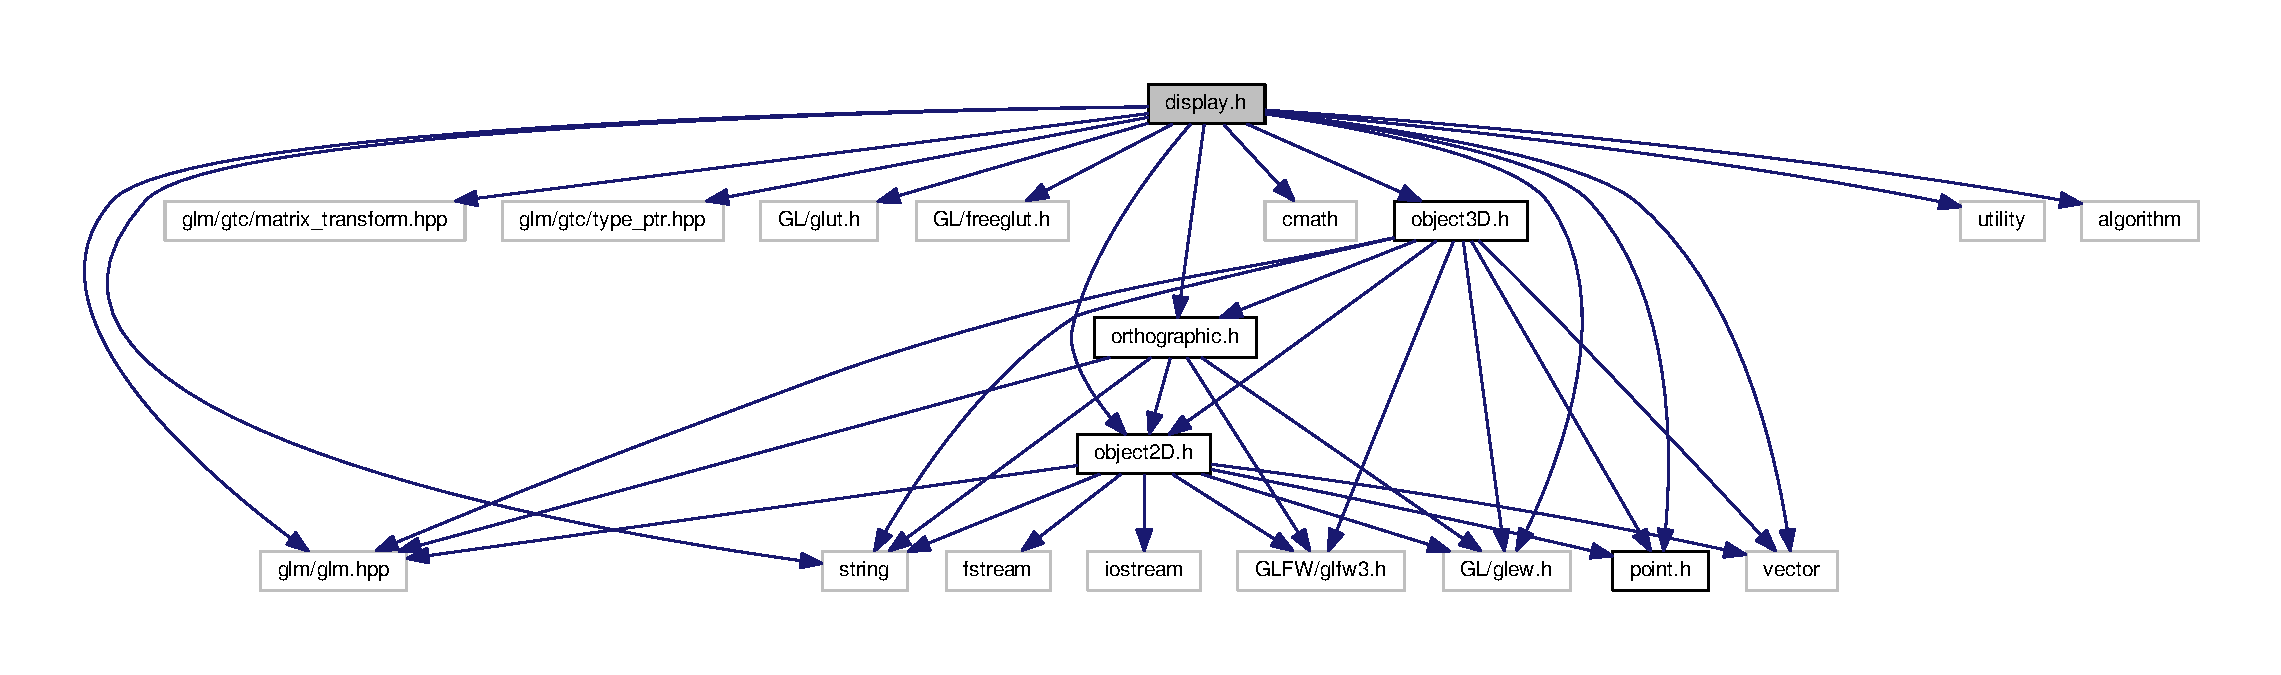
\includegraphics[width=350pt]{display_8h__incl}
\end{center}
\end{figure}
\subsection*{Functions}
\begin{DoxyCompactItemize}
\item 
void \mbox{\hyperlink{display_8h_a00fec396e195183623fac804494bae14}{initialise\+Glut}} ()
\item 
void \mbox{\hyperlink{display_8h_a1479f0135396d1da8b2e3b53bbf76bea}{draw\+Axis}} ()
\item 
void \mbox{\hyperlink{display_8h_afbed750fb4b47a35b89ed27013ef1ed7}{draw\+Axis\+Ortho}} ()
\item 
void \mbox{\hyperlink{display_8h_a9aefb21a75820e22cad4f3a9d8141c75}{keyboard}} (int key, int x, int y)
\item 
void \mbox{\hyperlink{display_8h_a15bb723be29642f3f7a7d65594e8e400}{make\+Line}} (glm\+::vec4 v1, glm\+::vec4 v2)
\item 
void \mbox{\hyperlink{display_8h_ac8bb3912a3ce86b15842e79d0b421204}{clear}} ()
\item 
void \mbox{\hyperlink{display_8h_a5a61d98384acd4ae597899ede878bc10}{clear\+Solid}} ()
\item 
void \mbox{\hyperlink{display_8h_a033cdabb8a11c8c51aac3d478c9d0a99}{render\+Wire3D}} ()
\item 
void \mbox{\hyperlink{display_8h_aabaa9df8411fb04f25d0d8c57d7676a1}{render\+Wire2D}} ()
\item 
void \mbox{\hyperlink{display_8h_a678b214934487d3899c70748e1ab13fa}{make\+Triangle}} (glm\+::vec4 a, glm\+::vec4 b, glm\+::vec4 c, glm\+::vec3 d)
\item 
glm\+::vec3 \mbox{\hyperlink{display_8h_ab9f5cf59a0083763b4f0129f4534b981}{cross}} (glm\+::vec4 a, glm\+::vec4 b)
\item 
void \mbox{\hyperlink{display_8h_a1755733190d5d1f71ab53b7a312a3afb}{render\+Solid3D}} ()
\item 
void \mbox{\hyperlink{display_8h_a67c0508c2a972cde8a032a30507ab113}{make\+Wire\+Frame}} (\mbox{\hyperlink{classobject3D}{object3D}} obj)
\item 
void \mbox{\hyperlink{display_8h_a1322fc6ed9d60edd489750625970eb69}{make\+Wire\+Frame}} (\mbox{\hyperlink{classobject2D}{object2D}} obj)
\item 
void \mbox{\hyperlink{display_8h_a166633547c25fb0e4a7e9ad3dec0b69e}{make\+Solid}} (\mbox{\hyperlink{classobject3D}{object3D}} obj)
\item 
void \mbox{\hyperlink{display_8h_acec548c51b36465faacca3216c5ba568}{make\+Orthographic}} (\mbox{\hyperlink{classorthographic}{orthographic}} obj)
\item 
void \mbox{\hyperlink{display_8h_a14c0faeb2d1eddd3150b5464cf3d5db3}{render\+Ortho}} ()
\item 
void \mbox{\hyperlink{display_8h_a9d848d1c4d6eb2d06560c2f9714b4bcb}{translated\+Render}} (glm\+::vec4 tr, glm\+::vec4 sca, int view\+\_\+number)
\item 
glm\+::vec4 \mbox{\hyperlink{display_8h_a385d494583bee0e23287d87de69da140}{change\+Coord}} (glm\+::vec4 ver, int view\+\_\+number)
\item 
void \mbox{\hyperlink{display_8h_aec2db323b595fa779c6a890f16343bd0}{make\+Isometric}} (\mbox{\hyperlink{classobject2D}{object2D}} obj)
\item 
void \mbox{\hyperlink{display_8h_a7aaceaab9a2c8d667c3a31dedc11dee2}{render\+Wire\+Iso}} ()
\end{DoxyCompactItemize}
\subsection*{Variables}
\begin{DoxyCompactItemize}
\item 
float \mbox{\hyperlink{display_8h_a8c76198699028c2a7e20377d7be0a1d8}{rX}}
\item 
float \mbox{\hyperlink{display_8h_a9bd9713cb50dc183d7081d9ec8e992d8}{rY}}
\item 
int \mbox{\hyperlink{display_8h_aa2e199e24ab9348b0514555b1e3ed642}{global\+\_\+argc}}
\item 
char $\ast$$\ast$ \mbox{\hyperlink{display_8h_a3e40e514937fc9a72d450b461a95dd75}{global\+\_\+argv}}
\item 
\mbox{\hyperlink{classobject3D}{object3D}} \mbox{\hyperlink{display_8h_a002476bba7e634fc8b1b756f41e30c4d}{rendering\+\_\+obj3D}}
\item 
\mbox{\hyperlink{classobject3D}{object3D}} \mbox{\hyperlink{display_8h_a27817ead792048f885eccb661151d3fb}{global\+\_\+obj3D}}
\item 
\mbox{\hyperlink{classobject2D}{object2D}} \mbox{\hyperlink{display_8h_a316011c2280afb4a7a56daedd08e55aa}{rendering\+\_\+obj2D}}
\item 
\mbox{\hyperlink{classobject2D}{object2D}} \mbox{\hyperlink{display_8h_acf4a02777bd541005052f8c0d54455bb}{global\+\_\+obj2D}}
\item 
\mbox{\hyperlink{classorthographic}{orthographic}} \mbox{\hyperlink{display_8h_aa6df6b74bbc619f915bf850d17f77309}{rendering\+\_\+obj\+Ortho}}
\item 
\mbox{\hyperlink{classorthographic}{orthographic}} \mbox{\hyperlink{display_8h_ac66b43d48c2773a7730009e20a6e952e}{global\+\_\+ortho\+Obj}}
\end{DoxyCompactItemize}


\subsection{Function Documentation}
\mbox{\Hypertarget{display_8h_a385d494583bee0e23287d87de69da140}\label{display_8h_a385d494583bee0e23287d87de69da140}} 
\index{display.\+h@{display.\+h}!change\+Coord@{change\+Coord}}
\index{change\+Coord@{change\+Coord}!display.\+h@{display.\+h}}
\subsubsection{\texorpdfstring{change\+Coord()}{changeCoord()}}
{\footnotesize\ttfamily glm\+::vec4 change\+Coord (\begin{DoxyParamCaption}\item[{glm\+::vec4}]{ver,  }\item[{int}]{view\+\_\+number }\end{DoxyParamCaption})}

function to rotate the coordinate system for orthographic views. \mbox{\Hypertarget{display_8h_ac8bb3912a3ce86b15842e79d0b421204}\label{display_8h_ac8bb3912a3ce86b15842e79d0b421204}} 
\index{display.\+h@{display.\+h}!clear@{clear}}
\index{clear@{clear}!display.\+h@{display.\+h}}
\subsubsection{\texorpdfstring{clear()}{clear()}}
{\footnotesize\ttfamily void clear (\begin{DoxyParamCaption}{ }\end{DoxyParamCaption})}

function to clear the glut screen in wireframe model \mbox{\Hypertarget{display_8h_a5a61d98384acd4ae597899ede878bc10}\label{display_8h_a5a61d98384acd4ae597899ede878bc10}} 
\index{display.\+h@{display.\+h}!clear\+Solid@{clear\+Solid}}
\index{clear\+Solid@{clear\+Solid}!display.\+h@{display.\+h}}
\subsubsection{\texorpdfstring{clear\+Solid()}{clearSolid()}}
{\footnotesize\ttfamily void clear\+Solid (\begin{DoxyParamCaption}{ }\end{DoxyParamCaption})}

function to clear the glut screen in the 3D models \mbox{\Hypertarget{display_8h_ab9f5cf59a0083763b4f0129f4534b981}\label{display_8h_ab9f5cf59a0083763b4f0129f4534b981}} 
\index{display.\+h@{display.\+h}!cross@{cross}}
\index{cross@{cross}!display.\+h@{display.\+h}}
\subsubsection{\texorpdfstring{cross()}{cross()}}
{\footnotesize\ttfamily glm\+::vec3 cross (\begin{DoxyParamCaption}\item[{glm\+::vec4}]{a,  }\item[{glm\+::vec4}]{b }\end{DoxyParamCaption})}

function to take the cross product of two vectors \mbox{\Hypertarget{display_8h_a1479f0135396d1da8b2e3b53bbf76bea}\label{display_8h_a1479f0135396d1da8b2e3b53bbf76bea}} 
\index{display.\+h@{display.\+h}!draw\+Axis@{draw\+Axis}}
\index{draw\+Axis@{draw\+Axis}!display.\+h@{display.\+h}}
\subsubsection{\texorpdfstring{draw\+Axis()}{drawAxis()}}
{\footnotesize\ttfamily void draw\+Axis (\begin{DoxyParamCaption}{ }\end{DoxyParamCaption})}

function to display the axis in the glut display window \mbox{\Hypertarget{display_8h_afbed750fb4b47a35b89ed27013ef1ed7}\label{display_8h_afbed750fb4b47a35b89ed27013ef1ed7}} 
\index{display.\+h@{display.\+h}!draw\+Axis\+Ortho@{draw\+Axis\+Ortho}}
\index{draw\+Axis\+Ortho@{draw\+Axis\+Ortho}!display.\+h@{display.\+h}}
\subsubsection{\texorpdfstring{draw\+Axis\+Ortho()}{drawAxisOrtho()}}
{\footnotesize\ttfamily void draw\+Axis\+Ortho (\begin{DoxyParamCaption}{ }\end{DoxyParamCaption})}

function to display axis in orthographic view \mbox{\Hypertarget{display_8h_a00fec396e195183623fac804494bae14}\label{display_8h_a00fec396e195183623fac804494bae14}} 
\index{display.\+h@{display.\+h}!initialise\+Glut@{initialise\+Glut}}
\index{initialise\+Glut@{initialise\+Glut}!display.\+h@{display.\+h}}
\subsubsection{\texorpdfstring{initialise\+Glut()}{initialiseGlut()}}
{\footnotesize\ttfamily void initialise\+Glut (\begin{DoxyParamCaption}{ }\end{DoxyParamCaption})}

function to initialize the glut window for display \mbox{\Hypertarget{display_8h_a9aefb21a75820e22cad4f3a9d8141c75}\label{display_8h_a9aefb21a75820e22cad4f3a9d8141c75}} 
\index{display.\+h@{display.\+h}!keyboard@{keyboard}}
\index{keyboard@{keyboard}!display.\+h@{display.\+h}}
\subsubsection{\texorpdfstring{keyboard()}{keyboard()}}
{\footnotesize\ttfamily void keyboard (\begin{DoxyParamCaption}\item[{int}]{key,  }\item[{int}]{x,  }\item[{int}]{y }\end{DoxyParamCaption})}

function to control the 3D figure rotation from the keyboard arrow keys \mbox{\Hypertarget{display_8h_aec2db323b595fa779c6a890f16343bd0}\label{display_8h_aec2db323b595fa779c6a890f16343bd0}} 
\index{display.\+h@{display.\+h}!make\+Isometric@{make\+Isometric}}
\index{make\+Isometric@{make\+Isometric}!display.\+h@{display.\+h}}
\subsubsection{\texorpdfstring{make\+Isometric()}{makeIsometric()}}
{\footnotesize\ttfamily void make\+Isometric (\begin{DoxyParamCaption}\item[{\mbox{\hyperlink{classobject2D}{object2D}}}]{obj }\end{DoxyParamCaption})}

\mbox{\Hypertarget{display_8h_a15bb723be29642f3f7a7d65594e8e400}\label{display_8h_a15bb723be29642f3f7a7d65594e8e400}} 
\index{display.\+h@{display.\+h}!make\+Line@{make\+Line}}
\index{make\+Line@{make\+Line}!display.\+h@{display.\+h}}
\subsubsection{\texorpdfstring{make\+Line()}{makeLine()}}
{\footnotesize\ttfamily void make\+Line (\begin{DoxyParamCaption}\item[{glm\+::vec4}]{v1,  }\item[{glm\+::vec4}]{v2 }\end{DoxyParamCaption})}

function to draw a line in the glut window between two points 
\begin{DoxyParams}{Parameters}
{\em v1} & takes first input vertex as glm vector \\
\hline
{\em v2} & takes second input vertex as glm vector \\
\hline
\end{DoxyParams}
\mbox{\Hypertarget{display_8h_acec548c51b36465faacca3216c5ba568}\label{display_8h_acec548c51b36465faacca3216c5ba568}} 
\index{display.\+h@{display.\+h}!make\+Orthographic@{make\+Orthographic}}
\index{make\+Orthographic@{make\+Orthographic}!display.\+h@{display.\+h}}
\subsubsection{\texorpdfstring{make\+Orthographic()}{makeOrthographic()}}
{\footnotesize\ttfamily void make\+Orthographic (\begin{DoxyParamCaption}\item[{\mbox{\hyperlink{classorthographic}{orthographic}}}]{obj }\end{DoxyParamCaption})}

function to actually setup call back functions for rendering orthographic views \mbox{\Hypertarget{display_8h_a166633547c25fb0e4a7e9ad3dec0b69e}\label{display_8h_a166633547c25fb0e4a7e9ad3dec0b69e}} 
\index{display.\+h@{display.\+h}!make\+Solid@{make\+Solid}}
\index{make\+Solid@{make\+Solid}!display.\+h@{display.\+h}}
\subsubsection{\texorpdfstring{make\+Solid()}{makeSolid()}}
{\footnotesize\ttfamily void make\+Solid (\begin{DoxyParamCaption}\item[{\mbox{\hyperlink{classobject3D}{object3D}}}]{obj }\end{DoxyParamCaption})}

function to actually setup call back functions for rendering 3D solid model \mbox{\Hypertarget{display_8h_a678b214934487d3899c70748e1ab13fa}\label{display_8h_a678b214934487d3899c70748e1ab13fa}} 
\index{display.\+h@{display.\+h}!make\+Triangle@{make\+Triangle}}
\index{make\+Triangle@{make\+Triangle}!display.\+h@{display.\+h}}
\subsubsection{\texorpdfstring{make\+Triangle()}{makeTriangle()}}
{\footnotesize\ttfamily void make\+Triangle (\begin{DoxyParamCaption}\item[{glm\+::vec4}]{a,  }\item[{glm\+::vec4}]{b,  }\item[{glm\+::vec4}]{c,  }\item[{glm\+::vec3}]{d }\end{DoxyParamCaption})}

function to draw triangle between 3 points and make surface from the normal 
\begin{DoxyParams}{Parameters}
{\em a} & first vertex \\
\hline
{\em b} & second vertex \\
\hline
{\em c} & third vertex \\
\hline
{\em d} & normal vector to the surface \\
\hline
\end{DoxyParams}
\mbox{\Hypertarget{display_8h_a67c0508c2a972cde8a032a30507ab113}\label{display_8h_a67c0508c2a972cde8a032a30507ab113}} 
\index{display.\+h@{display.\+h}!make\+Wire\+Frame@{make\+Wire\+Frame}}
\index{make\+Wire\+Frame@{make\+Wire\+Frame}!display.\+h@{display.\+h}}
\subsubsection{\texorpdfstring{make\+Wire\+Frame()}{makeWireFrame()}\hspace{0.1cm}{\footnotesize\ttfamily [1/2]}}
{\footnotesize\ttfamily void make\+Wire\+Frame (\begin{DoxyParamCaption}\item[{\mbox{\hyperlink{classobject3D}{object3D}}}]{obj }\end{DoxyParamCaption})}

function to actually setup call back functions for rendering 3D wireframe object \mbox{\Hypertarget{display_8h_a1322fc6ed9d60edd489750625970eb69}\label{display_8h_a1322fc6ed9d60edd489750625970eb69}} 
\index{display.\+h@{display.\+h}!make\+Wire\+Frame@{make\+Wire\+Frame}}
\index{make\+Wire\+Frame@{make\+Wire\+Frame}!display.\+h@{display.\+h}}
\subsubsection{\texorpdfstring{make\+Wire\+Frame()}{makeWireFrame()}\hspace{0.1cm}{\footnotesize\ttfamily [2/2]}}
{\footnotesize\ttfamily void make\+Wire\+Frame (\begin{DoxyParamCaption}\item[{\mbox{\hyperlink{classobject2D}{object2D}}}]{obj }\end{DoxyParamCaption})}

function to actually setup call back functions for rendering 2D wireframe object \mbox{\Hypertarget{display_8h_a14c0faeb2d1eddd3150b5464cf3d5db3}\label{display_8h_a14c0faeb2d1eddd3150b5464cf3d5db3}} 
\index{display.\+h@{display.\+h}!render\+Ortho@{render\+Ortho}}
\index{render\+Ortho@{render\+Ortho}!display.\+h@{display.\+h}}
\subsubsection{\texorpdfstring{render\+Ortho()}{renderOrtho()}}
{\footnotesize\ttfamily void render\+Ortho (\begin{DoxyParamCaption}{ }\end{DoxyParamCaption})}

function to display the orthographic views on the glut screen \mbox{\Hypertarget{display_8h_a1755733190d5d1f71ab53b7a312a3afb}\label{display_8h_a1755733190d5d1f71ab53b7a312a3afb}} 
\index{display.\+h@{display.\+h}!render\+Solid3D@{render\+Solid3D}}
\index{render\+Solid3D@{render\+Solid3D}!display.\+h@{display.\+h}}
\subsubsection{\texorpdfstring{render\+Solid3\+D()}{renderSolid3D()}}
{\footnotesize\ttfamily void render\+Solid3D (\begin{DoxyParamCaption}{ }\end{DoxyParamCaption})}

function to render 3D solid model with surface shading \mbox{\Hypertarget{display_8h_aabaa9df8411fb04f25d0d8c57d7676a1}\label{display_8h_aabaa9df8411fb04f25d0d8c57d7676a1}} 
\index{display.\+h@{display.\+h}!render\+Wire2D@{render\+Wire2D}}
\index{render\+Wire2D@{render\+Wire2D}!display.\+h@{display.\+h}}
\subsubsection{\texorpdfstring{render\+Wire2\+D()}{renderWire2D()}}
{\footnotesize\ttfamily void render\+Wire2D (\begin{DoxyParamCaption}{ }\end{DoxyParamCaption})}

function to render 2D wireframe model \mbox{\Hypertarget{display_8h_a033cdabb8a11c8c51aac3d478c9d0a99}\label{display_8h_a033cdabb8a11c8c51aac3d478c9d0a99}} 
\index{display.\+h@{display.\+h}!render\+Wire3D@{render\+Wire3D}}
\index{render\+Wire3D@{render\+Wire3D}!display.\+h@{display.\+h}}
\subsubsection{\texorpdfstring{render\+Wire3\+D()}{renderWire3D()}}
{\footnotesize\ttfamily void render\+Wire3D (\begin{DoxyParamCaption}{ }\end{DoxyParamCaption})}

function to render 3D wireframe model \mbox{\Hypertarget{display_8h_a7aaceaab9a2c8d667c3a31dedc11dee2}\label{display_8h_a7aaceaab9a2c8d667c3a31dedc11dee2}} 
\index{display.\+h@{display.\+h}!render\+Wire\+Iso@{render\+Wire\+Iso}}
\index{render\+Wire\+Iso@{render\+Wire\+Iso}!display.\+h@{display.\+h}}
\subsubsection{\texorpdfstring{render\+Wire\+Iso()}{renderWireIso()}}
{\footnotesize\ttfamily void render\+Wire\+Iso (\begin{DoxyParamCaption}{ }\end{DoxyParamCaption})}

\mbox{\Hypertarget{display_8h_a9d848d1c4d6eb2d06560c2f9714b4bcb}\label{display_8h_a9d848d1c4d6eb2d06560c2f9714b4bcb}} 
\index{display.\+h@{display.\+h}!translated\+Render@{translated\+Render}}
\index{translated\+Render@{translated\+Render}!display.\+h@{display.\+h}}
\subsubsection{\texorpdfstring{translated\+Render()}{translatedRender()}}
{\footnotesize\ttfamily void translated\+Render (\begin{DoxyParamCaption}\item[{glm\+::vec4}]{tr,  }\item[{glm\+::vec4}]{sca,  }\item[{int}]{view\+\_\+number }\end{DoxyParamCaption})}

function to correctly translate the orthographic views for display 

\subsection{Variable Documentation}
\mbox{\Hypertarget{display_8h_aa2e199e24ab9348b0514555b1e3ed642}\label{display_8h_aa2e199e24ab9348b0514555b1e3ed642}} 
\index{display.\+h@{display.\+h}!global\+\_\+argc@{global\+\_\+argc}}
\index{global\+\_\+argc@{global\+\_\+argc}!display.\+h@{display.\+h}}
\subsubsection{\texorpdfstring{global\+\_\+argc}{global\_argc}}
{\footnotesize\ttfamily int global\+\_\+argc}

\mbox{\Hypertarget{display_8h_a3e40e514937fc9a72d450b461a95dd75}\label{display_8h_a3e40e514937fc9a72d450b461a95dd75}} 
\index{display.\+h@{display.\+h}!global\+\_\+argv@{global\+\_\+argv}}
\index{global\+\_\+argv@{global\+\_\+argv}!display.\+h@{display.\+h}}
\subsubsection{\texorpdfstring{global\+\_\+argv}{global\_argv}}
{\footnotesize\ttfamily char$\ast$$\ast$ global\+\_\+argv}

\mbox{\Hypertarget{display_8h_acf4a02777bd541005052f8c0d54455bb}\label{display_8h_acf4a02777bd541005052f8c0d54455bb}} 
\index{display.\+h@{display.\+h}!global\+\_\+obj2D@{global\+\_\+obj2D}}
\index{global\+\_\+obj2D@{global\+\_\+obj2D}!display.\+h@{display.\+h}}
\subsubsection{\texorpdfstring{global\+\_\+obj2D}{global\_obj2D}}
{\footnotesize\ttfamily \mbox{\hyperlink{classobject2D}{object2D}} global\+\_\+obj2D}

\mbox{\Hypertarget{display_8h_a27817ead792048f885eccb661151d3fb}\label{display_8h_a27817ead792048f885eccb661151d3fb}} 
\index{display.\+h@{display.\+h}!global\+\_\+obj3D@{global\+\_\+obj3D}}
\index{global\+\_\+obj3D@{global\+\_\+obj3D}!display.\+h@{display.\+h}}
\subsubsection{\texorpdfstring{global\+\_\+obj3D}{global\_obj3D}}
{\footnotesize\ttfamily \mbox{\hyperlink{classobject3D}{object3D}} global\+\_\+obj3D}

\mbox{\Hypertarget{display_8h_ac66b43d48c2773a7730009e20a6e952e}\label{display_8h_ac66b43d48c2773a7730009e20a6e952e}} 
\index{display.\+h@{display.\+h}!global\+\_\+ortho\+Obj@{global\+\_\+ortho\+Obj}}
\index{global\+\_\+ortho\+Obj@{global\+\_\+ortho\+Obj}!display.\+h@{display.\+h}}
\subsubsection{\texorpdfstring{global\+\_\+ortho\+Obj}{global\_orthoObj}}
{\footnotesize\ttfamily \mbox{\hyperlink{classorthographic}{orthographic}} global\+\_\+ortho\+Obj}

\mbox{\Hypertarget{display_8h_a316011c2280afb4a7a56daedd08e55aa}\label{display_8h_a316011c2280afb4a7a56daedd08e55aa}} 
\index{display.\+h@{display.\+h}!rendering\+\_\+obj2D@{rendering\+\_\+obj2D}}
\index{rendering\+\_\+obj2D@{rendering\+\_\+obj2D}!display.\+h@{display.\+h}}
\subsubsection{\texorpdfstring{rendering\+\_\+obj2D}{rendering\_obj2D}}
{\footnotesize\ttfamily \mbox{\hyperlink{classobject2D}{object2D}} rendering\+\_\+obj2D}

\mbox{\Hypertarget{display_8h_a002476bba7e634fc8b1b756f41e30c4d}\label{display_8h_a002476bba7e634fc8b1b756f41e30c4d}} 
\index{display.\+h@{display.\+h}!rendering\+\_\+obj3D@{rendering\+\_\+obj3D}}
\index{rendering\+\_\+obj3D@{rendering\+\_\+obj3D}!display.\+h@{display.\+h}}
\subsubsection{\texorpdfstring{rendering\+\_\+obj3D}{rendering\_obj3D}}
{\footnotesize\ttfamily \mbox{\hyperlink{classobject3D}{object3D}} rendering\+\_\+obj3D}

\mbox{\Hypertarget{display_8h_aa6df6b74bbc619f915bf850d17f77309}\label{display_8h_aa6df6b74bbc619f915bf850d17f77309}} 
\index{display.\+h@{display.\+h}!rendering\+\_\+obj\+Ortho@{rendering\+\_\+obj\+Ortho}}
\index{rendering\+\_\+obj\+Ortho@{rendering\+\_\+obj\+Ortho}!display.\+h@{display.\+h}}
\subsubsection{\texorpdfstring{rendering\+\_\+obj\+Ortho}{rendering\_objOrtho}}
{\footnotesize\ttfamily \mbox{\hyperlink{classorthographic}{orthographic}} rendering\+\_\+obj\+Ortho}

\mbox{\Hypertarget{display_8h_a8c76198699028c2a7e20377d7be0a1d8}\label{display_8h_a8c76198699028c2a7e20377d7be0a1d8}} 
\index{display.\+h@{display.\+h}!rX@{rX}}
\index{rX@{rX}!display.\+h@{display.\+h}}
\subsubsection{\texorpdfstring{rX}{rX}}
{\footnotesize\ttfamily float rX}

\mbox{\Hypertarget{display_8h_a9bd9713cb50dc183d7081d9ec8e992d8}\label{display_8h_a9bd9713cb50dc183d7081d9ec8e992d8}} 
\index{display.\+h@{display.\+h}!rY@{rY}}
\index{rY@{rY}!display.\+h@{display.\+h}}
\subsubsection{\texorpdfstring{rY}{rY}}
{\footnotesize\ttfamily float rY}


\hypertarget{object2D_8h}{}\section{object2\+D.\+h File Reference}
\label{object2D_8h}\index{object2\+D.\+h@{object2\+D.\+h}}


This file contains the class \mbox{\hyperlink{classobject2D}{object2D}}, which is used to model a 2D figure.  


{\ttfamily \#include $<$G\+L/glew.\+h$>$}\newline
{\ttfamily \#include $<$G\+L\+F\+W/glfw3.\+h$>$}\newline
{\ttfamily \#include $<$glm/glm.\+hpp$>$}\newline
{\ttfamily \#include $<$iostream$>$}\newline
{\ttfamily \#include $<$fstream$>$}\newline
{\ttfamily \#include \char`\"{}point.\+h\char`\"{}}\newline
{\ttfamily \#include $<$vector$>$}\newline
{\ttfamily \#include $<$string$>$}\newline
Include dependency graph for object2\+D.\+h\+:\nopagebreak
\begin{figure}[H]
\begin{center}
\leavevmode
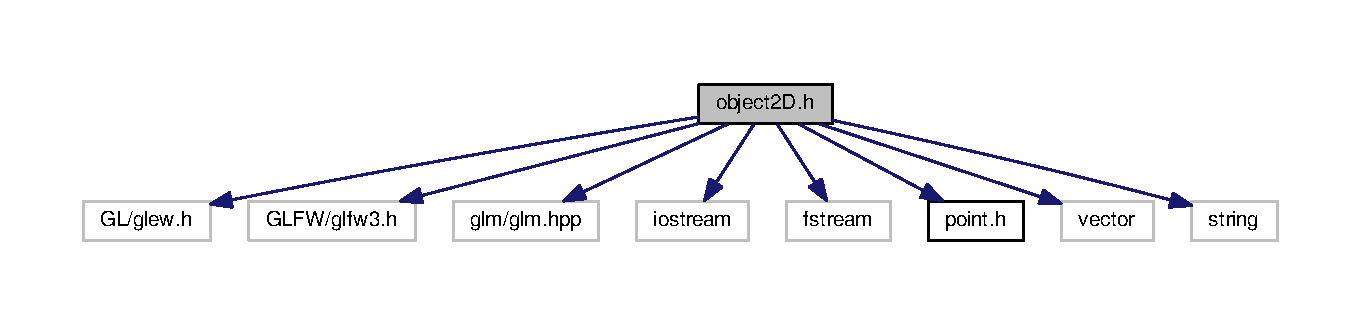
\includegraphics[width=350pt]{object2D_8h__incl}
\end{center}
\end{figure}
This graph shows which files directly or indirectly include this file\+:\nopagebreak
\begin{figure}[H]
\begin{center}
\leavevmode
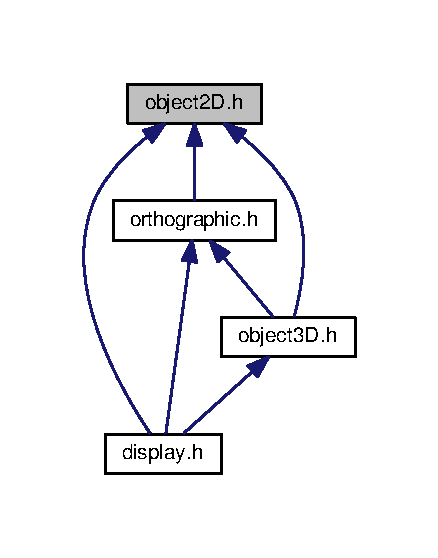
\includegraphics[width=210pt]{object2D_8h__dep__incl}
\end{center}
\end{figure}
\subsection*{Classes}
\begin{DoxyCompactItemize}
\item 
class \mbox{\hyperlink{classobject2D}{object2D}}
\end{DoxyCompactItemize}


\subsection{Detailed Description}
This file contains the class \mbox{\hyperlink{classobject2D}{object2D}}, which is used to model a 2D figure. 


\hypertarget{object3D_8h}{}\section{object3\+D.\+h File Reference}
\label{object3D_8h}\index{object3\+D.\+h@{object3\+D.\+h}}


This file contains the class \mbox{\hyperlink{classobject3D}{object3D}} which is used to model a 3D object.  


{\ttfamily \#include $<$G\+L/glew.\+h$>$}\newline
{\ttfamily \#include $<$G\+L\+F\+W/glfw3.\+h$>$}\newline
{\ttfamily \#include $<$glm/glm.\+hpp$>$}\newline
{\ttfamily \#include $<$string$>$}\newline
{\ttfamily \#include $<$vector$>$}\newline
{\ttfamily \#include \char`\"{}point.\+h\char`\"{}}\newline
{\ttfamily \#include \char`\"{}object2\+D.\+h\char`\"{}}\newline
{\ttfamily \#include \char`\"{}orthographic.\+h\char`\"{}}\newline
Include dependency graph for object3\+D.\+h\+:\nopagebreak
\begin{figure}[H]
\begin{center}
\leavevmode
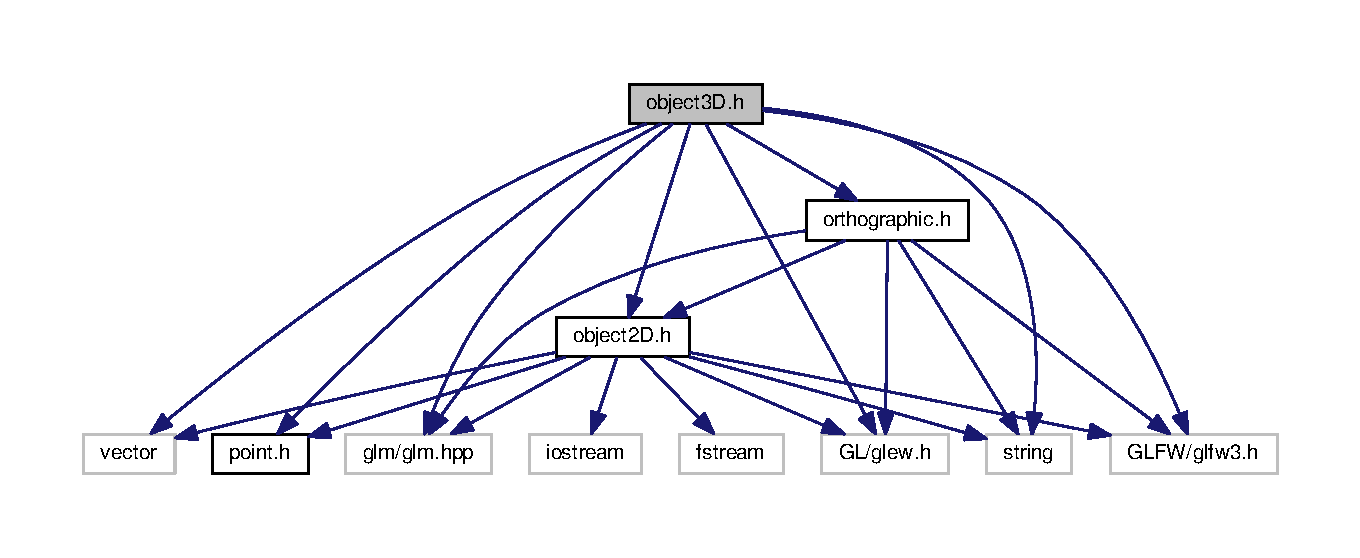
\includegraphics[width=350pt]{object3D_8h__incl}
\end{center}
\end{figure}
This graph shows which files directly or indirectly include this file\+:\nopagebreak
\begin{figure}[H]
\begin{center}
\leavevmode
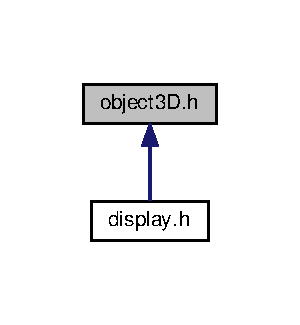
\includegraphics[width=144pt]{object3D_8h__dep__incl}
\end{center}
\end{figure}
\subsection*{Classes}
\begin{DoxyCompactItemize}
\item 
class \mbox{\hyperlink{classobject3D}{object3D}}
\end{DoxyCompactItemize}


\subsection{Detailed Description}
This file contains the class \mbox{\hyperlink{classobject3D}{object3D}} which is used to model a 3D object. 


\hypertarget{orthographic_8h}{}\section{orthographic.\+h File Reference}
\label{orthographic_8h}\index{orthographic.\+h@{orthographic.\+h}}


This file contains the class orthographic which is used to model orthographic projections of a 3D object.  


{\ttfamily \#include $<$G\+L/glew.\+h$>$}\newline
{\ttfamily \#include $<$G\+L\+F\+W/glfw3.\+h$>$}\newline
{\ttfamily \#include $<$glm/glm.\+hpp$>$}\newline
{\ttfamily \#include \char`\"{}object2\+D.\+h\char`\"{}}\newline
{\ttfamily \#include $<$string$>$}\newline
Include dependency graph for orthographic.\+h\+:\nopagebreak
\begin{figure}[H]
\begin{center}
\leavevmode
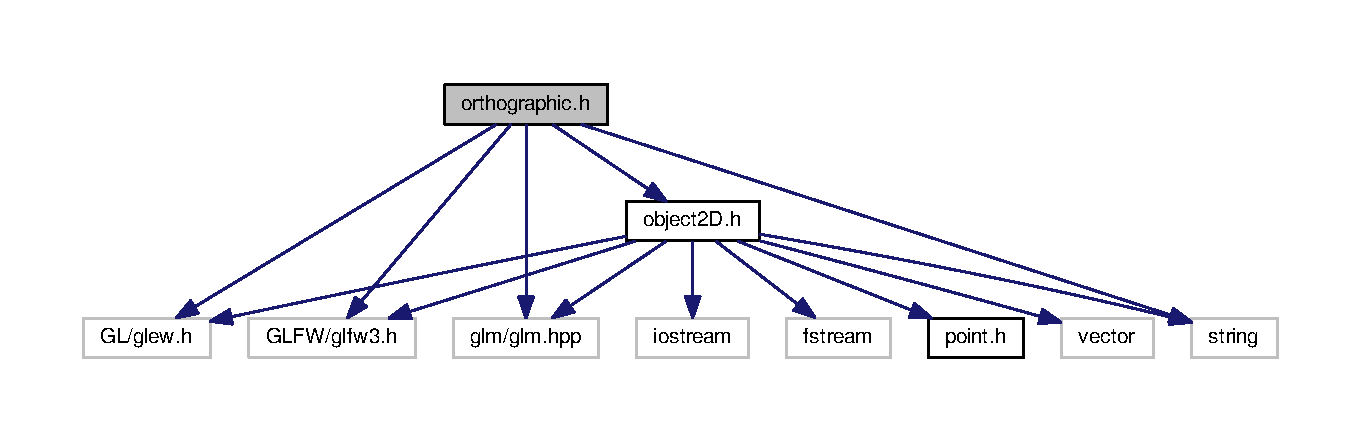
\includegraphics[width=350pt]{orthographic_8h__incl}
\end{center}
\end{figure}
This graph shows which files directly or indirectly include this file\+:\nopagebreak
\begin{figure}[H]
\begin{center}
\leavevmode
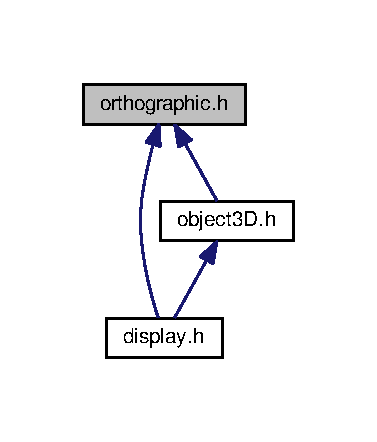
\includegraphics[width=181pt]{orthographic_8h__dep__incl}
\end{center}
\end{figure}
\subsection*{Classes}
\begin{DoxyCompactItemize}
\item 
class \mbox{\hyperlink{classorthographic}{orthographic}}
\end{DoxyCompactItemize}


\subsection{Detailed Description}
This file contains the class orthographic which is used to model orthographic projections of a 3D object. 


\hypertarget{point_8h}{}\section{point.\+h File Reference}
\label{point_8h}\index{point.\+h@{point.\+h}}


This file contains the classes used to model various geometric objects such as point, line and a plane.  


This graph shows which files directly or indirectly include this file\+:\nopagebreak
\begin{figure}[H]
\begin{center}
\leavevmode
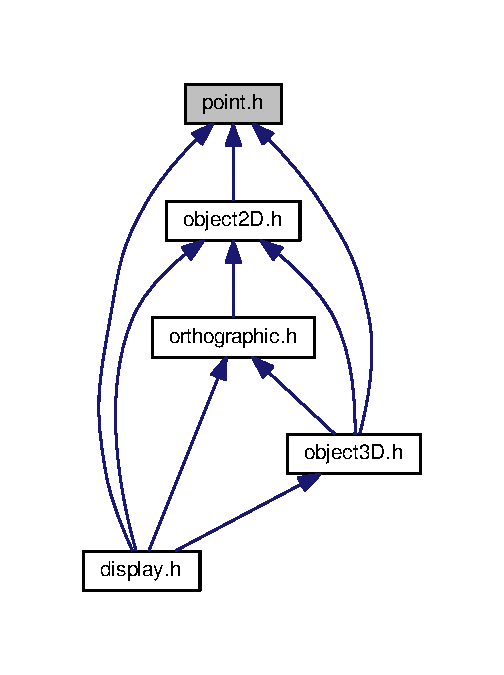
\includegraphics[width=242pt]{point_8h__dep__incl}
\end{center}
\end{figure}
\subsection*{Classes}
\begin{DoxyCompactItemize}
\item 
class \mbox{\hyperlink{classpoint}{point}}
\item 
class \mbox{\hyperlink{classline}{line}}
\item 
class \mbox{\hyperlink{classplane}{plane}}
\end{DoxyCompactItemize}


\subsection{Detailed Description}
This file contains the classes used to model various geometric objects such as point, line and a plane. 


%--- End generated contents ---

% Index
\backmatter
\newpage
\phantomsection
\clearemptydoublepage
\addcontentsline{toc}{chapter}{Index}
\printindex

\end{document}
